% --------------------------------------------------------------
% This is all preamble stuff that you don't have to worry about.
% Head down to where it says "Start here"
% --------------------------------------------------------------
 
\documentclass[12pt]{article}
 
\usepackage[margin=1in]{geometry} 
\usepackage{amsmath,amsthm,amssymb}
\usepackage[margin=1in]{geometry} 
\usepackage{amsmath,amsthm,amssymb}
\usepackage[utf8]{inputenc}
\usepackage[T1]{fontenc} %escribe lo del teclado
\usepackage[utf8]{inputenc} %Reconoce algunos símbolos
\usepackage{lmodern} %optimiza algunas fuentes
\usepackage{graphicx}
\graphicspath{ {images/} }
\usepackage{hyperref} % Uso de links
\usepackage{float}
\date{}

\newcommand{\N}{\mathbb{N}}
\newcommand{\Z}{\mathbb{Z}}
 
\newenvironment{theorem}[2][Theorem]{\begin{trivlist}
\item[\hskip \labelsep {\bfseries #1}\hskip \labelsep {\bfseries #2.}]}{\end{trivlist}}
\newenvironment{lemma}[2][Lemma]{\begin{trivlist}
\item[\hskip \labelsep {\bfseries #1}\hskip \labelsep {\bfseries #2.}]}{\end{trivlist}}
\newenvironment{exercise}[2][Exercise]{\begin{trivlist}
\item[\hskip \labelsep {\bfseries #1}\hskip \labelsep {\bfseries #2.}]}{\end{trivlist}}
\newenvironment{problem}[2][Problem]{\begin{trivlist}
\item[\hskip \labelsep {\bfseries #1}\hskip \labelsep {\bfseries #2.}]}{\end{trivlist}}
\newenvironment{question}[2][Question]{\begin{trivlist}
\item[\hskip \labelsep {\bfseries #1}\hskip \labelsep {\bfseries #2.}]}{\end{trivlist}}
\newenvironment{corollary}[2][Corollary]{\begin{trivlist}
\item[\hskip \labelsep {\bfseries #1}\hskip \labelsep {\bfseries #2.}]}{\end{trivlist}}

\newenvironment{solution}{\begin{proof}[Solution]}{\end{proof}}
 
\begin{document}
 
% --------------------------------------------------------------
%                         Start here
% --------------------------------------------------------------
 
\title{Trabajo 2 Programación}
\author{Víctor Manuel Arroyo Martín\\ %replace with your name
Aprendizaje Automático}

\maketitle
\section{Ejercicio sobre la complejidad de H y el ruido}
1.- El resultado gráfico es el siguiente:
\begin{figure}[h]
\centering
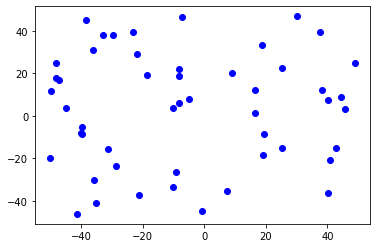
\includegraphics[scale=0.45]{Images/Ej1a.png} 
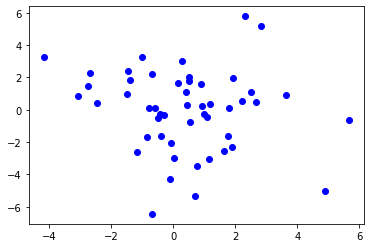
\includegraphics[scale=0.45]{Images/Ej1b.png} 
\caption{A la izquierda con simula unif y a la derecha con simula gaus}
\label{etiqueta}
\end{figure}
\\
2.- Ahora pide generar 100 nuevos puntos y una recta. \\\\
a) Así, he creado una gráfica con la recta y la nube de puntos clasificada, como se pedía:
\begin{figure}[h]
\centering
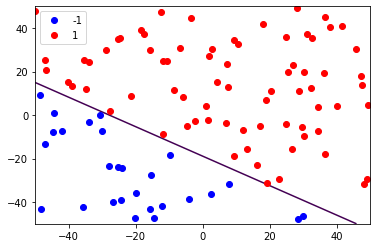
\includegraphics[scale=0.75]{Images/Ej2a.png} 
\caption{Recta y puntos con sus etiquetas}
\label{etiqueta}
\end{figure}
\\
Como se puede ver en la gráfica, todos están bien clasificados: etiqueta 1 por encima de la recta y -1 por debajo. \\\\
b) Ahora tenemos que meter ruido tanto en las etiquetas 1 como en -1 (un 10$ \% $ en ambas), quedando la gráfica de la siguiente manera:
\begin{figure}[h]
\centering
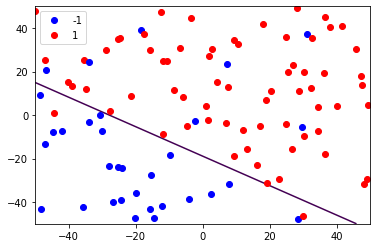
\includegraphics[scale=0.75]{Images/Ej2b.png} 
\caption{Recta y puntos con sus etiquetas y ruido}
\label{etiqueta}
\end{figure}
\\
Para comprobarlo numéricamente he hecho el porcentaje de mal clasificadas: hay un 6'25$\%$ de etiquetas negativas mal clasificadas y un 10'29$\%$ de positivas, como cabía esperar.\\\\
c) En este último apartado nos pedían hacer lo mismo que en el 2b) pero con distintas funciones. Las gráficas resultantes son:\\\\
$ \bullet $ Para f(x,y) = $ (x - 10)^{2} + (y - 20)^{2} - 400 $\\
\begin{figure}[h]
\centering
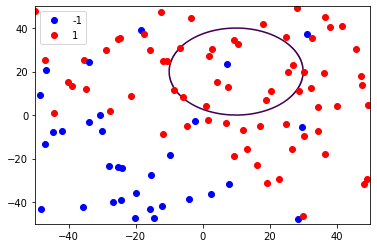
\includegraphics[scale=0.75]{Images/Ej2ca.png} 
\caption{Función y puntos con sus etiquetas y ruido}
\label{etiqueta}
\end{figure}
\\
Que da los siguientes errores:
\begin{center}
ERROR en la funcion de las negativas: 96.875\\
ERROR en la funcion de las positivas: 19.11764705882353
\end{center}

$ \bullet $ Para f(x,y) = $ 0'5(x + 10)^{2} + (y - 20)^{2} - 400 $\\
\begin{figure}[h]
\centering
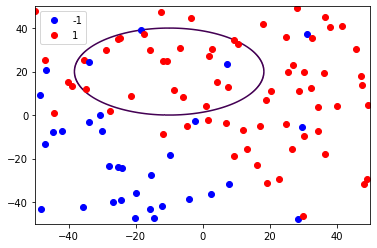
\includegraphics[scale=0.75]{Images/Ej2cb.png} 
\caption{Función y puntos con sus etiquetas y ruido}
\label{etiqueta}
\end{figure}
\\
Que da los siguientes errores:
\begin{center}
ERROR en la funcion de las negativas: 93.75\\
ERROR en la funcion de las positivas: 29.41176470588235
\end{center}

$ \bullet $ Para f(x,y) = $ 0'5(x - 10)^{2} + (y - 20)^{2} - 400 $
\begin{figure}[h]
\centering
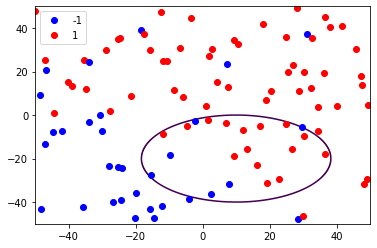
\includegraphics[scale=0.75]{Images/Ej2cc.png} 
\caption{Función y puntos con sus etiquetas y ruido}
\label{etiqueta}
\end{figure}
\\
Con los siguientes errores:
\begin{center}
ERROR en la funcion de las negativas: 84.375\\
ERROR en la funcion de las positivas: 22.058823529411764
\end{center}

$ \bullet $ Para f(x,y) = $ y - 20x^{2} - 5x + 3 $
\begin{figure}[h]
\centering
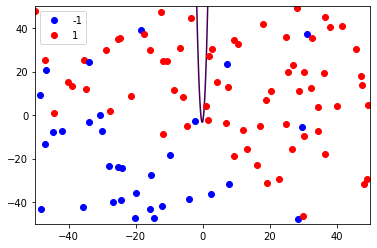
\includegraphics[scale=0.75]{Images/Ej2cd.png} 
\caption{Función y puntos con sus etiquetas y ruido}
\label{etiqueta}
\end{figure}
\\
Que por último da los siguientes errores:
\begin{center}
ERROR en la funcion de las negativas: 0.0 \\
ERROR en la funcion de las positivas: 100.0
\end{center}
En todas se han usado los porcentajes de mal clasificadas.\\
Como hemos podido apreciar en los errores, estas funciones más complejas no son mejores clasificadoras que la lineal ya que en este caso, la nube de puntos se ajusta mejor a una línea que a una parábola o elipse. Así, modificar las etiquetas del problema llevaría a transformarlo en un problema totalmente distinto del que estamos estudiando.

\section{Modelos Lineales}
a)\\
1.- Con el vector 0 me da 444 iteraciones y el vector de pesos w=[-2129, 44.85508745, 17.01070298]. Para comprobar que no depende del punto de inicio, lo he ejecutado 10 veces y ha dado exactamente el mismo resultado.
\begin{figure}[h]
\centering
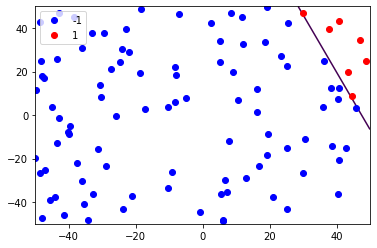
\includegraphics[scale=0.75]{Images/Ej2a1.png} 
\caption{Recta resultante para el vector de inicio 0}
\label{etiqueta}
\end{figure}
\\\\\\\\\\\\\\\\\\\\\
Luego, para vectores de inicio aleatorios, me da como resultado 818'1 iteraciones del algoritmo. Esto lo que nos dice es que depende mucho del vector de inicio que elijamos el que converja antes o después pero como hemos visto antes, el mismo punto de inicio da siempre el mismo resultado.\\\\
2.- En este apartado lo que pide es hacer lo mismo pero esta vez con ruido. Lo que ha ocurrido es que el algoritmo nunca para y no da una buena recta de clasificación. Esto es debido a que el PLA lo que hace es recorrer punto a punto y ver si está bien etiquetado. Si no lo está, modifica la recta para que esté bien etiquetado. Debido a esto, el PLA solo para cuando la nuve de puntos se ajusta de forma perfecta a una recta, lo cual no es el caso de este apartado: es imposible ajustale una recta. Por ello, cicla intentando etiquetar bien todos los puntos con tan solo una recta.
\begin{figure}[h]
\centering
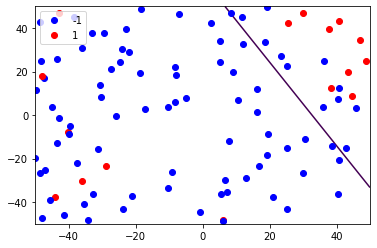
\includegraphics[scale=0.75]{Images/Ej2a2.png} 
\caption{Recta resultante para la nube con ruido}
\label{etiqueta}
\end{figure}
\\
He puesto 1200 iteraciones como máximo y de media con vectores aleatorios de inicio me ha dado, efectivamente, 1200 iteraciones y una recta "mala", por así decirlo. \\\\
b)\\
1.- Mediante simula recta he generado una recta aleatoria y he etiquetado en el cuadrado [0,2] los 100 puntos aleatorios. Luego le he aplicado Regresión Logística para calcular la recta que clasifica con las restricciones pedidas en el apartado.\\\\
2.- Con todo lo anterior he obtenido: \\
\begin{figure}[h]
\centering
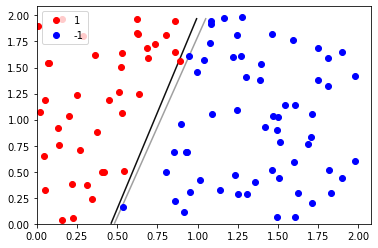
\includegraphics[scale=0.75]{Images/Ej2b1.png} 
\caption{En negro, la recta resultante de RL y en gris la que etiqueta}
\label{etiqueta}
\end{figure}
\\
Número de iteraciones: 378\\
Vector de pesos w=[4.08863438, -8.85381745,  2.39486174]\\
Error dentro de la muestra:  0.08196087430087234\\
Este error (claculado mediante la fórmula vista para RL en la teoría) es muy bajo así que podemos concluir que el algoritmo de Regresión Logística es muy buen clasificador.\\\\
Para terminar he hecho 1000 iteraciones de 100 puntos nuevos y los he etiquetado con la misma recta y 1000 puntos nuevos etiquetados también, para obtener el error fuera de la muestra. Con ello, he conseguido los siguientes errores:\\
\begin{center}
Error fuera de la muestra para una muestra de 1000 puntos 0.09515339596934251\\
Error medio fuera de la muestra en 1000 iteraciones de 100 puntos de muestra aleatorios 0.09615966690382156
\end{center}
Que siguen siendo bastante bajos.\\
\section{BONUS}
a) El problema de clasificación binaria podría ser el siguiente:\\
Dada una muestra de los dígitos 4 y 8 manuscritos donde nos dan la información de su intensidad de gris promedio y su simetría, ajustar un modelo de clasificación oportuno para encontrar la función solución g que mejor clasifique estos puntos.\\
b) El modelo que he elegido es el de gradiente descendiente estocástico con un learning rate del 0.01, 500 iteraciones máximas y un minibach de 32.\\
1) Nos pide generar gráficos de las nubes de puntos del training y del test: \\
\begin{figure}[h]
\centering
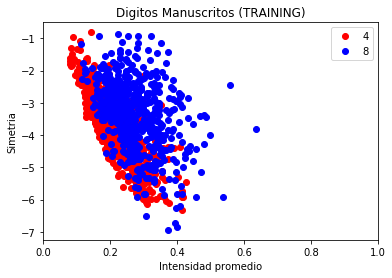
\includegraphics[scale=0.45]{Images/EjB1.png} 
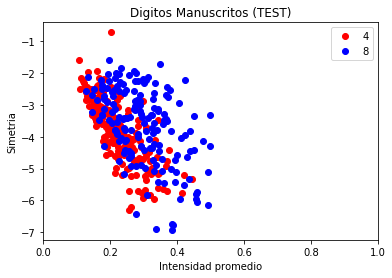
\includegraphics[scale=0.45]{Images/EjB2.png} 
\caption{A la izquierda el training, a la derecha el test}
\label{etiqueta}
\end{figure}
\\
2) La gráfica resultante de aplicar sgd sobre el training con las características dichas al principio es:\\
\begin{figure}[h]
\centering
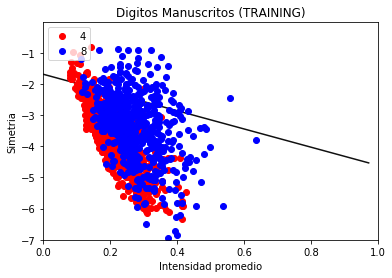
\includegraphics[scale=0.75]{Images/EjB3.png} 
\caption{Recta resultante del gradiente descendiente estocástico}
\label{etiqueta}
\end{figure}
\\
Y los errores cuadráticos medios de éste son:
\begin{center}
Error en el training:  0.9346675302326157\\
Error en el test:  0.9655569705832843
\end{center}
Que como vemos, son bastante altos así que el modelo no es capaz de ajustar correctamente la nube de puntos. Por ello, nos piden hacer mejora con PLA-Pocket. Este algoritmo se basa en ejecutar un número de iteraciones dado la recta mediante PLA y guardando siempre el menor error y la mejor recta, que será el resultado del algoritmo. Con ello, se ha conseguido mejorar mucho la recta y ha disminuído considerablemente el error de esta, quedando la siguiente gráfica y errores:\\
\begin{figure}[h]
\centering
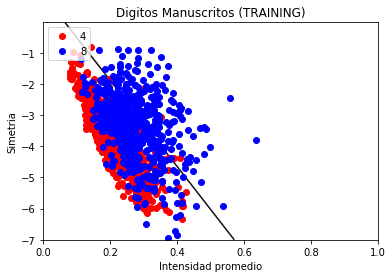
\includegraphics[scale=0.75]{Images/EjB4.png} 
\caption{Recta resultante del gradiente descendiente estocástico}
\label{etiqueta}
\end{figure}
\\
Con errores 
\begin{center}
Error en la muestra:  0.2554438860971524\\
Error fuera de la muestra (test):  0.30327868852459017
\end{center}
c) Por último nos piden calcular una cota para el $E_{out}$. Siguiendo la teoría he usado la siguiente desigualdad de Hoeffding:
\begin{center}
$ E_{out}(h) \leq E_{in} + \sqrt{\frac{1}{2N}log \frac{2}{\delta}} $
\end{center}
Donde se asegura que será así con una probabilidad de 1-$\delta$, en este caso con probabilidad del 95$\%$ ya que $\delta$=0.05 y N es el tamaño de la muestra. Para que la desigualdad esté basada en $E_{test}$, sólo hay que sustituír $E_{in}$ por $E_{test}$. Así, obtenemos las siguientes cotas:\\
\begin{center}
Cota para el $E_{out}$ basado en el $E_{in}$:  0.2947472815017796 \\
Cota para $E_{out}$ basado en el $E_{test}$:  0.34258208392921735
\end{center}
La mejor cota es la del $E_{test}$ pues es lo más cercano al $E_{out}$ que tenemos y sabemos que en general nunca va a sobrepasar ese valor.







% --------------------------------------------------------------
%     You don't have to mess with anything below this line.
% --------------------------------------------------------------
 
\end{document}